\section{Aufgabenstellung}


Wir haben uns zum Ziel gesetzt, einen vollwertigen Musikempfehlungsdienst zu entwickeln, welcher auf Basis von Linked Data arbeitet. Inspiriert ist dies durch den Internetdienst Musicbrainz\footnote{\url{http://www.musicbrainz.org/}}. Dabei handelt es sich um eine offene Musik-Enzyklopädie, die zahlreiche Informationen zu Musikern und Bands anbietet. Dazu zählen Informationen wie ein kurzer Abstract, eine Discographie, externe Links, eine Liste aller aktueller und ehemaliger Mitglieder der Band etc. Sucht man auf Musicbrainz zum Beispiel nach der Band \glqq Queens of the Stone Age\grqq, sieht man dort, dass Josh Homme das einzige verbliebene Gründungsmitglied der Band ist. Mit einem Klick auf den Namen wird man zur Seite von Josh Homme weitergeleitet. Dort sieht man unter Anderem in welchen anderen Bands er gespielt hat und kann sich wiederum Informationen zu diesen ansehen.

\paragraph{} Der Benutzer kann also ausgehend von einem Interpreten weitere entdecken. Genau diese Möglichkeit soll auch MusicMashup bieten. Der Benutzer gibt den Names eines Interpreten ein und bekommt passend zu diesem Empfehlungen. Klickt er eine dieser Empfehlungen an, werden ihm wiederum für diesen Interpreten Empfehlungen angezeigt. 


\paragraph{} Erweitert wird dies durch zusätzliche Informationen und Funktionen. Die wohl wichtigste Zusatzfunktion ist ein eingebundener Spotify-Player, welcher die Möglichkeit bietet, sich direkt Musik des jeweiligen Künstlers anzuhören. Darüber hinaus wird eine Liste mit anstehenden Konzerten ausgegeben, sowie weiterführende Links, eine Bildergalerie und ein kurzer Abstract über den Artist. Damit der Benutzer nachvollziehen kann, wie er von einem Interpreten zum Nächsten gekommen ist, wird im Header der Seite eine Liste der zuvor betrachteten Interpreten angezeigt.

\subsection{Technische Grundlagen des Servers}

MusicMashup ist als so genannte Web-App realisiert und präsentiert sich dem Benutzer als interaktive Website, die er aus seinem Browser nutzen kann.

Die programmatische Grundlage von MusicMashup bildet ein in Python geschriebener 
HTTP-Server basierend auf dem \textit{cherrypy}-Modul\footnote{\url{http://www.cherrypy.org/}}. Dieser Server wertet die Nutzeranfrage aus, führt die entsprechenden Abfragen durch und liefert die daraus generierten Empfehlungen mittels der Template-Engine mako\footnote{\cite{http://www.makotemplates.org/}} als Website aus. 

\subsection{Klassenstruktur}


\paragraph{}Das System besteht aus vier Klassen: \textit{MusicMashupServer}, \textit{MusicMashupArtist}, \textit{MusicMashupParser} und \textit{MusicMashupPagerank} (siehe Abb. X).


\begin{figure}[ht!]
\centering
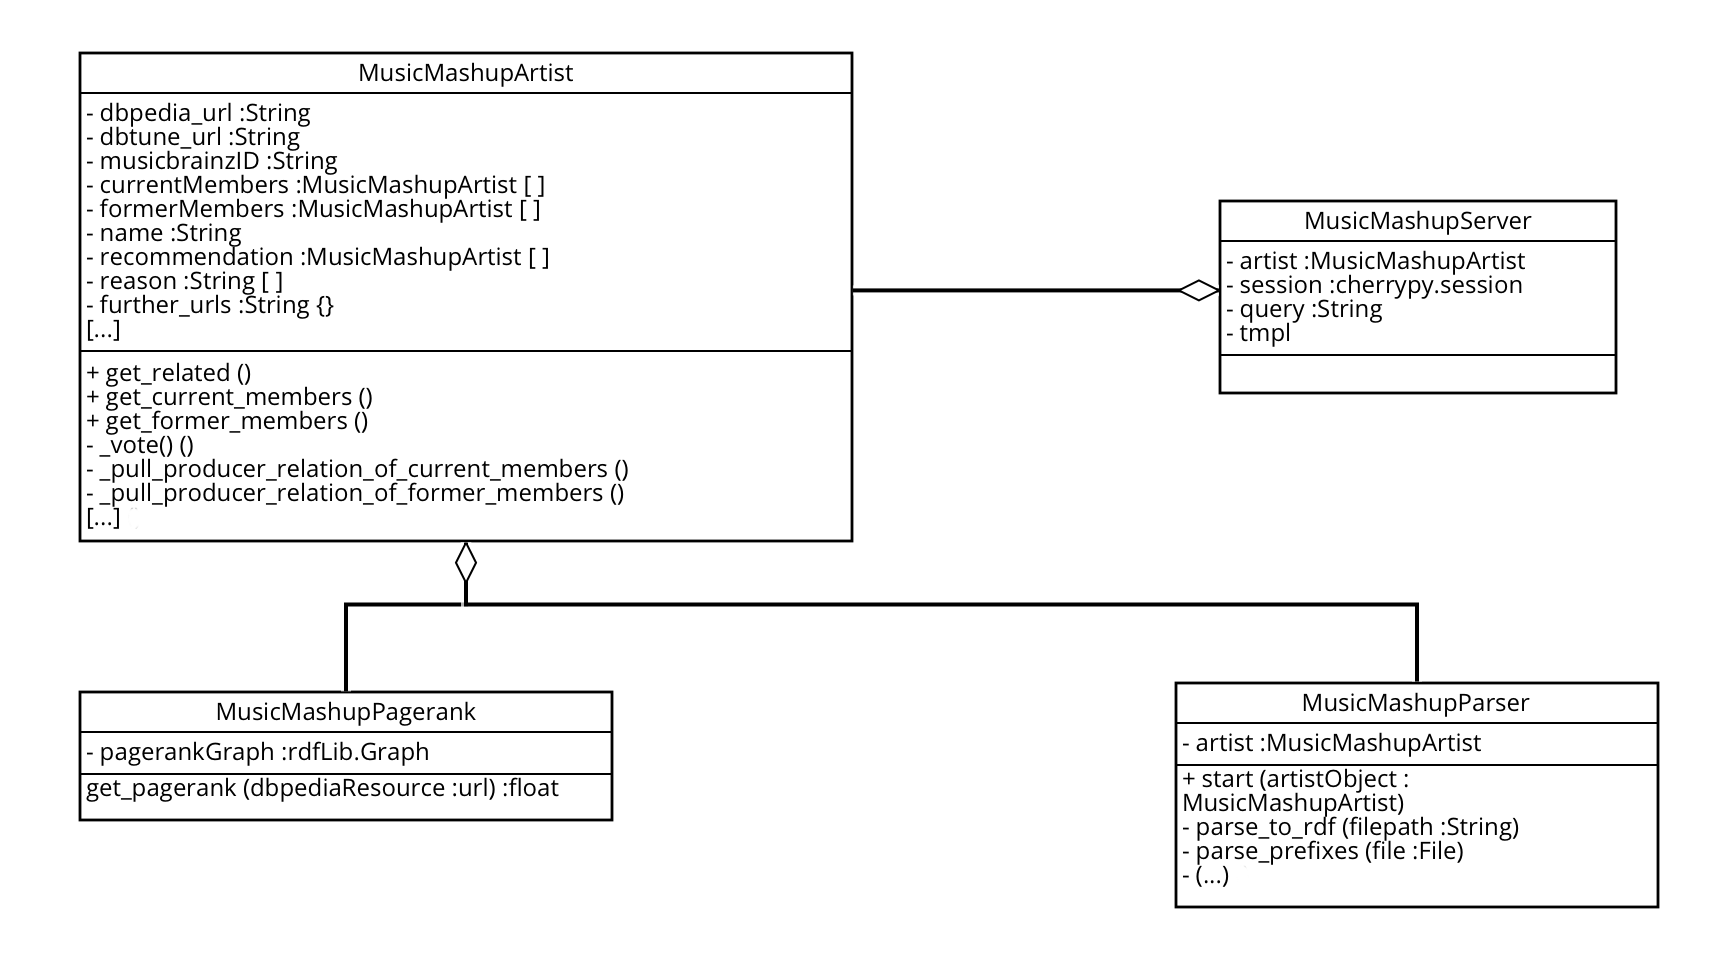
\includegraphics[width=137mm]{bilder/klassendiagramm.png}
\caption{Klassendiagramm der beschriebenen Klassen von MusicMashup \label{overflow}}
\end{figure}

% loest funktionen aus???
\paragraph{Server} Die Klasse \textit{MusicMashupServer} stellt den Web-Server bereit und löst bei einem Aufruf der Anwendung weitere Funktionen aus. Wird nach einem Interpreten gesucht, wird für diesen Interpreten ein Objekt vom Typ MusicMashupArtist erstellt. Diesem wird entweder die Suchanfrage oder aber eine aus einer Empfehlung stammende DBpedia-URL übergeben, sollte eine Empfehlung angeklickt worden sein. Die eigentliche Programmlogik geschieht dann in diesem Objekt. Nachdem diese ausgeführt wurde, wird anschließend das HTML-Dokument gerendert und an den Browser ausgeliefert.


\paragraph{Artist} Die Klasse \textit{MusicMashupArtist} dient als Repräsentation eines Artists. Sie implementiert alle Abfragen, mittels derer Informationen über einen Artist gefunden werden und speichert diese. Darüber hinaus stellt sie Funktionen bereit, die es dem HTML-Template ermöglichen, diese Informationen abzufragen, um sie anschließend anzeigen zu lassen.


\paragraph{Parser} Die Klasse \textit{MusicMashupParser} ist eine simple Implementierung eines Parser, der die Informationen, die zu den Artists gefunden werden, in eine Turtle-Datei (.ttl) schreibt. Bei Turtle handelt es sich um eine Syntax des RDF-Formats, welche eine Repräsentation eines RDF-Graphen in Textform ermöglicht \cite{turtle}. Das Parsen geschieht aus zwei Gründen: erstens liegt nicht jede der Datenquellen in Form von Linked Data vor. Der Parser überführt die Informationen in eine solche Turtle-Datei und ermöglicht so eine Bereitstellung der Daten als Linked Data.  Zweitens kann beim Aufruf eines Artists überprüft werden, ob bereits eine Turtle-Datei existiert, in dem die Informationen zur Verfügung stehen. Falls ja, können diese aus der Datei geladen werden, was zu einer deutlichen Verringerung der Ladezeit führt.


\paragraph{Pagerank} Die Klasse \textit{MusicMashupPagerank} wird einmalig beim Aufruf der Anwendung instanziert und dient als Schnittstelle zum Dump der DBpedia-Pageranks, welche in einen Graphen geladen werden und somit zum Abfragen bereitstehen.

\subsection{Datensätze}

\paragraph{Musicbrainz} Musicbrainz verwendet IDs, um Artists eindeutig zu identifizieren. Diese IDs wurden von vielen anderen Musikdiensten zur Identifikation von Artists übernommen. Um diese zu erhalten, wird eine Anfrage auf DBtune\footnote{\url{http://www.dbtune.org/musicbrainz/}} gestellt. Dabei handelt es sich um ein Linked Data Mapping der Musicbrainz Datenbank. Bei einer erfolgreichen Abfrage erhält das System die Musicbrainz-ID und über \texttt{owl:sameAs} den Link zur entsprechenden DBpedia-Ressource. Da DBtune jedoch nicht vollständig ist (zum Beispiel enthält DBtune keinen Eintrag für die Band \glqq Them Crooked Vultures\grqq), wird als Fallback ein Linked Data Dump der Musicbrainz-Datenbank benutzt. Zwar gibt es in vielen Fällen, in denen es keinen Eintrag auf DBtune gibt, einen Eintrag im Musicbrainz-Dump, jedoch hält der Dump keinen Verweis auf DBpedia, weswegen er schlussendlich nur als Fallback zum Einsatz kommt.

\paragraph{DBpedia} Als Hauptdatenquelle kommt DBpedia zum Einsatz. Von der DBpedia erhält unser System zu einem Interpreten den Abstract, eine Liste der aktuellen und ehemaligen Bandmitglieder sowie ein Thumbnail. Um die bereits vorher genannten zusätzlichen Informationen und Funktionen bereitzustellen, musste auf Datenquellen zurückgegriffen werden, die nicht im Linked Data Format vorliegen. Dazu gehören Spotify für den Musikplayer, Songkick\footnote{\url{http://www.songkick.com/developer/}} für zukünftige Konzerte und Echonest\footnote{\url{http://developer.echonest.com/}}. Echonest dient einerseits als Schnittstelle zu den anderen APIs, andererseits liefert es auch einen sogenannten \glqq Familiarity\grqq-Wert, welcher benutzt wird, um die Relevanz der gefundenen Empfehlungen zu bewerten (dazu später mehr).

\paragraph{Commons} Weiterhin kommen die DBpedia-Commons\footnote{\url{http://commons.dbpedia.org/}} sowie ein Dump der DBpedia-Pageranks \cite{dbpedia-graphmeasures} zum Einsatz. DBpedia-Commons stellt die Wikimedia-Commons als Linked Data bereit. Diese werden benutzt, um zu einer Band Bilder in einer Bildergallerie bereit zu stellen, sollten welche vorliegen. 
Der Dump der DBpedia-Pageranks, welcher von der Semantic-Technologies-Forschungsgruppe des Hasso-Plattner-Instituts bereitgestellt wurde, hält für jede DBpedia-Ressource einen Eintrag über ihren Pagerank. MusicMashup verwendet diesen Dump, reduziert auf Ressourcen mit dem \texttt{rdf:type} \texttt{Band}, \texttt{MusicalArtist} bzw. \texttt{Artist}.

\subsection{Funktionsweise}


Beim erstmaligen Aufruf von MusicMashup wird dem Benutzer eine einfach gestaltete Startseite präsentiert, auf der mittels eines Eingabefelds nach einem Artist  suchen kann, zu dem er sich Empfehlungen geben lassen möchte.


% Bild: Startseite

\subsubsection{Finden von Informationen zum Künstler}
Der vom Benutzer eingegebene Name wird zunächst in Titlecase überführt. Das bedeutet, dass alle Wortanfangsbuchstaben der Eingabe in Großbuchstaben überführt werden, außer es handelt sich um Artikel oder Präpositionen. Wir haben bei unserer Arbeit feststellen können, dass sich somit mehr als 95\% aller Künstler zuverlässig finden lassen.
Anschließend wird auf DBtune nach einer Ressource gesucht, deren \texttt{rdfs:label} mit der Eingabe des Nutzers übereinstimmt und die außerdem als \texttt{rdf:type} den Eintrag \texttt{mo:MusicArtist} hat. Wird eine Ressource gefunden, erhält das System die Musicbrainz-ID des Artists sowie den Link zur DBpedia-Ressource.

Für den Fall, dass sich ein Artist nicht auf DBtune finden lässt, wird im Musicbrainz-Dump nach dem Artist gesucht. Statt \texttt{rdfs:label} kommt hier \texttt{foaf:name} zum Einsatz. Da im Musicbrainz-Dump kein Verweis auf den entsprechenden DBpedia-Eintrag vorhanden ist, muss auf der DBpedia selbst nach der entsprechenden Ressource gesucht werden.

\begin{figure}[ht!]
\centering
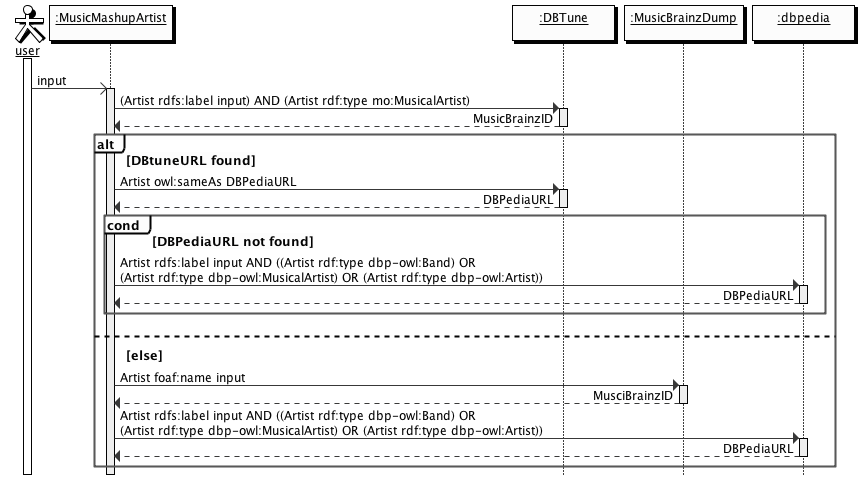
\includegraphics[width=137mm]{bilder/sequenzdiagramm.png}
\caption{Zum gesuchten Künstler wird eine Ressource gefunden \label{overflow}}
\end{figure}


\subsubsection{Suche nach Recommendations}
Ist der Link zur DBpedia-Ressource des jeweiligen Künstlers vorhanden, kann gezielt nach Empfehlungen gesucht werden. Dazu werden zunächst alle aktuellen sowie ehemaligen Mitglieder der Band via \texttt{dbpprop:currentMembers} oder \texttt{dbpedia-owl:bandMembers}  bzw. \texttt{dbpprop:pastMembers} oder \texttt{dbpedia-owl:formerBandMember} abgefragt. Im Anschluss werden für jedes so gefundene Mitglied folgende Relationen überprüft: die Membership-Relation (s.o), die Producer-Relation (\texttt{dbprop:producer} oder \texttt{dbpedia-owl:producer}), die Composer-Relation (\texttt{dbpedia-owl:composer}) und die Writer-Relation (\texttt{dbpedia-owl:writer} oder \texttt{dbpprop:writer}). Grundsätzlich wird für jede Relation nach Bands oder Künstlern gesucht, in denen ein aktuelles oder ehemaliges Mitglied der Band zur Zeit spielt, gespielt hat bzw. nach Bands, für die ein aktuelles oder ehemaliges Mitglied der Band produziert oder einen Song geschrieben bzw. komponiert hat. 

\subsubsection{Auswerten der Empfehlungen}
Wird bei einer dieser Abfragen eine Empfehlung gefunden, gibt es zwei Möglichkeiten: ist der gefundene Artist noch nicht in der Liste der empfohlenen Artists enthalten, wird er der Liste samt des Grundes, warum er empfohlen wird, hinzugefügt. Sollte der gefundene Interpret bereits in der Liste enthalten sein, wird diesem Artist lediglich der Grund hinzugefügt, weshalb er gefunden wurde.  % vllt umbauen?


Nachdem alle Relationen überprüft wurden, wird mittels eines Voting-Algorithmus über die Relevanz der einzelnen Empfehlungen entschieden. Dafür wird der Familiarity-Wert genutzt, den die Echonest-API bereit stellt, sowie die DBpedia-Pageranks. Die Echonest-Familiarity ist ein von Echonest errechneter Wert, der aussagt, wie bekannt die Band ist.\cite{echonest_familiarity}
% anhand? bekannt ggf. ersetzen?

\paragraph{} Des weiteren wird jeder Relation ein Faktor zugeordnet, der mit in die Berechnung einfließt. Diese Faktoren haben die Aufgabe, die Wichtigkeit der Relationen untereinander zu bewerten. Die Membership-Relation für aktuelle Bands hat den höchsten Faktor, gefolgt von der Membership-Relation für ehemalige Bands, der Producer-Relation und der Writer- und der Composer-Relation, welche gleichwertig sind. Geht diese Relation von einem aktuellen Mitglied der Band aus, so ist der Faktor doppelt so hoch wie für ein ehemaliges Mitglied. Am Ende werden der DBpedia-Pagerank, die Echonest-Familiarity und der Relationsfaktor miteinander multipliziert. Die Empfehlung mit dem höchsten Wert steht in der Liste der Vorschläge oben und die mit dem niedrigsten Wert unten.
Nach Abschluss des Votings wird der Parser gestartet, welcher alle gefundenen Informationen für einen Artist in eine Turtle-Datei schreibt. % ehemalige band? 2x am Ende

\paragraph{} Wurden alle Schritte erledigt, kann die Seite gerendert und ausgegeben werden (siehe Abb. x).


% Bild einer fertigen Seite